\section{Inferring Signalling Frequency and Power Consumption from Network Traces}\label{sec:network:network_traces}
All participating stakeholders, i.e. network operators, hardware vendors, and application developers, need to assess the impact of potential changes of parts of the mobile network, e.g. change of network parameters, introduction of new hardware or modification of applications, on their considered \glspl{KPI} without rolling out changes to the production network.
To this end, we propose specific metrics in order to quantify the impact of changes on the network on the considered \gls{KPI}.
We introduce an algorithm to infer metrics from application traffic measurements, network parameters and power and signalling configurations.
In \refsec{sec:network:network_traces:performance_evaluation} we present the algorithm and methods to describe the relevant metrics.
Then, in \refsec{sec:network:network_traces:numerical_results}, we use the proposed methodology to evaluate the impact of various network configurations on four popular applications.

\subsection{Inferring State Transitions and Deriving Metrics}\label{sec:network:network_traces:performance_evaluation}
A \gls{UE}’s firmware triggers \gls{RRC} state transitions based on application traffic.
While solutions exist to capture RRC state transitions on specific hardware~\cite{zayas2010} they are not available for all modern smartphone platforms.
Other options to measure the required information include using costly hardware and use specific \glspl{UE}, usually not available to researchers and application developers.
This prevents the developers from evaluating the effect of their applications on the overall health
of the network.
Consequently, they can not take measures to prevent the harmful behaviour of their applications.
However, it is possible to infer the \gls{RRC} state transitions for a given packet trace if the network configuration is known.

First, we describe the setup used to capture network packet traces for arbitrary apps.
Then, we give an algorithm to infer the \gls{RRC} state transitions for a given packet trace.
Based on these state transitions, we can calculate the number of signalling messages generated
by the packet trace. 
Finally, we use the information on when which \gls{RRC} state was entered to calculate the power drain of the \gls{UE}’s radio interface.

\subsubsection*{Measurement Procedure and Setup}\label{sec:network:network_traces:performance_evaluation:measurement}
To investigate the behaviour of the application under study, we capture traffic during a typical use of the application on a \emph{Samsung Galaxy SII} smartphone.
The smartphone runs the Android operating system and is connected to the \gls{3G} network of a major German network operator.
To obtain the network packet traces we use the \texttt{tcpdump} application.
This application requires \emph{root} privileges which are obtained by rooting the device and installing the custom \emph{cyanogenmod} ROM \footnote{\url{http://www.cyanogenmod.org}, Accessed: November, \(21^{st}\) 2015}.
Once \texttt{tcpdump} is installed and running, we start the application under study and capture packet traces while the application is running.
Then, the \emph{android debugging bridge} is used to copy the traces to a workstation.
The traces contain \gls{IP} packets embedded in Linux Cooked Captures.
We require the \gls{IP} packets, thus we extracted the \gls{IP} packets which are used during the analysis to follow.

\subsubsection*{Inferring Network State}\label{sec:network:network_traces:performance_evaluation:inferring_network_state}
In this section we study the influence of the application traffic on \gls{RRC} state transitions and signalling messages.
Since \gls{RRC} state transitions can not be captured using commonly available tools, we introduce an algorithm to infer \gls{RRC} state transitions from \gls{IP} packet traces.
Using this algorithm we analyse the \gls{RRC} state transition frequency and signalling message load for the Two State Model and Three State Model.

Traffic below the network layer can not be measured without specific equipment which interfaces with the proprietary firmware of the \gls{UE} and is often out of reach for developers interested in assessing the impact of their applications on the network.
Based on the Two State and Three State models introduced in \refsec{sec:network:background:umts_rrc}, we process \texttt{tcpdump} captures of the application traffic.
However, it should be noted that this method is not restricted to a specific network model, but can be extended to any other network model as well.
Using these captures, we extract the timestamps when \gls{IP} packets are sent or received.
Furthermore, we require the timer values of the transition from \gls{RRC_DCH} state to \gls{RRC_FACH} state, \gls{TDCH}, and the timer for the transition between \gls{RRC_FACH} and \gls{RRC_idle} states, \gls{TFACH}.
Based on these informations \refalg{alg:network:network_traces:performance_evaluation:inferring_network_state:inference_algorithm} infers the timestamps of state transitions according to the \gls{3GPP} specification \cite{3GPP_RRC_Spec} for the Three State Model.
This algorithm can be simplified to also work for the Two State Model. 
Alternatively, a method to post process the results of the algorithm to obtain results for the Two State Model is given at the end of this section.
The algorithm first computes the inter-arrival times of all packets.
Then, each timestamp is considered.
If the \gls{UE} is currently in \gls{RRC_idle} state, a state transition to \gls{RRC_DCH} occurs at the moment the packet is sent or received.
If the inter-arrival time exceeds the \gls{TDCH} timer the \gls{UE} transitions to \gls{RRC_FACH} \gls{TDCH} seconds after the packet was sent or received.
Similarly, if the inter-arrival time exceeds both the \gls{TDCH} and \gls{TFACH} timers a state transition to \gls{RRC_idle} occurs \gls{TDCH} seconds after the state transition to \gls{RRC_FACH}.

\begin{algorithm}
  \begin{algorithmic}
    \Require{Packet arrival timestamps \emph{ts}\\
    \gls{RRC_DCH} to \gls{RRC_FACH} timer \gls{TDCH}\\
    \gls{RRC_FACH} to \gls{RRC_idle} timer \gls{TFACH}}
    \Ensure{Times of state transition \emph{state\_time}\\
    New states after state transitions \emph{state}}
    \State \texttt{interarrival(i)} $\leftarrow$ \emph{ts}(i+1) - \emph{ts}(i)
    \State \texttt{index} $\leftarrow 0$
    \ForAll{ts(i)}
      \If{\texttt{state(index)} = \gls{RRC_idle}}
        \State \texttt{index} $\leftarrow$ \texttt{index} + 1
        \State \texttt{state(index)} $\leftarrow$ \gls{RRC_DCH}
        \State \texttt{state\_time(index)} $\leftarrow$ ts(i)
      \EndIf
      \If{\texttt{interarrival}(i-1) $> \gls{TDCH}$}
        \State \texttt{index} $\leftarrow$ \texttt{index} + 1
        \State \texttt{state(index)} $\leftarrow$ \gls{RRC_FACH}
        \State \texttt{state\_time(index)} $\leftarrow$ ts(i) $+ \gls{TDCH}$
      \EndIf
      \If{\texttt{interarrival}(i-1) $> \gls{TDCH} + \gls{TFACH}$}
        \State \texttt{index} $\leftarrow$ \texttt{index} + 1
        \State \texttt{state(index)} $\leftarrow$ \gls{RRC_idle}
        \State \texttt{state\_time(index)} $\leftarrow$ ts(i) $+ \gls{TDCH} + \gls{TFACH}$
      \EndIf
    \EndFor
  \end{algorithmic}
  \caption{Inferring \headershortacr{RRC} state transitions based on \headershortacr{IP} timestamps.}
  \label{alg:network:network_traces:performance_evaluation:inferring_network_state:inference_algorithm}
\end{algorithm}

Decreasing power drain of their devices is always a goal of \gls{UE} vendors.
A straightforward way to achieve this, if only the wellbeing of the \gls{UE} is considered, is to transition from \gls{RRC_DCH} state to \gls{RRC_idle} as soon as no additional data is ready for sending.
While this transition is not directly available in the 3GPP specification for the \gls{RRC} protocol \cite{3GPP_RRC_Spec}, a \gls{UE} may reset the connection, effectively transitioning from any state to \gls{RRC_idle}.
This behaviour can be modeled using the Two State Model introduced in \refsec{sec:network:background:umts_rrc}.

State transitions for the Two State Model can be calculated using a similar algorithm.
Alternatively, the behaviour of the Two State Model can be emulated using \refalg{alg:network:network_traces:performance_evaluation:inferring_network_state:inference_algorithm} if \gls{TFACH} is set to \SI{0}{\second} and all state transitions to \gls{RRC_FACH} are removed in a post processing step.

\subsubsection*{Calculating Signalling Frequency and Power Drain}\label{sec:network:network_traces:calculating_metrics}

\begin{table}
\centering
  \caption{Number of signalling messages per \headershortacr{RRC} state transition perceived at the \headershortacr{RNC} \cite{3GPP_RRC_Spec}.}
  \label{tab:network:network_traces:calculating_metrics:signalling_messages}
\begin{tabular}{lccc}
	\toprule
    from/to & \gls{RRC_idle} & \gls{RRC_FACH} & \gls{RRC_DCH}\\
    \midrule
    \gls{RRC_idle} & -- & 28 & 32\\
    \gls{RRC_FACH} & 22 & -- & 6\\
    \gls{RRC_DCH} & 25 & 5 & --\\
    \bottomrule    
	\end{tabular}
\end{table}

In reality, the number of state transitions is not the metric of most importance if network signalling is to be evaluated.
Each state transition results in a number of \gls{RRC} messages between the \gls{UE} and different network components.
For this study we consider the number of messages observed at the \gls{RNC}, which can be found in \cite{3GPP_RRC_Spec} and is summarized in \reftab{tab:network:network_traces:calculating_metrics:signalling_messages}.
It can be seen that transitions from or to the \gls{RRC_idle} state are especially expensive in terms of number of messages sent or received.
This is due to the fact that upon entering or leaving the \gls{RRC_idle} state, authentication has to be performed. 
Note that for the Two State Model only transitions from or to the \gls{RRC_idle} state occur.
This results in the fact that for the same network packet trace the number of signalling messages occurring in the Two State Model is generally higher than in the Three State Model.
To obtain the total number of signalling messages, we weight the number of state transitions with the number of messages sent per state transitions.
Then, we average the number of state transitions over the measurement duration to obtain a metric for the signalling load at the \gls{RNC}, i.e. the \gls{SF}.
The inference algorithm does not differentiate between state changes caused by upstream or downstream traffic.
State changes caused by downstream traffic usually generate some additional signalling messages, as paging is involved.
The inference algorithm can easily be enhanced to support this behaviour.
However, the results discussed in the next section would only change quantitatively.
Furthermore, the algorithm can be adapted to new networking models or other numbers of signalling messages sent per state transition.

\begin{table}
  \centering
  \caption{Power consumption of the \headershortacr{UE} radio interface depending on current \headershortacr{RRC} state \cite{Qian2011a}.}
  \label{tab:network:network_traces:calculating_metrics:power_consumption}  
  \begin{tabular}{lc}
  	\toprule
    \gls{RRC} State & Power Consumption\\
    \midrule
    \gls{RRC_idle} & \SI{0}{\milli\watt}\\
    \gls{RRC_FACH} & \SI{650}{\milli\watt}\\
    \gls{RRC_DCH} & \SI{800}{\milli\watt}\\
    \bottomrule
  \end{tabular}
\end{table}

From a users point of view, the signalling message frequency is of little importantance.
The user is interested in a low power drain as this increases the battery life of the device.
To calculate the battery life, we use the time when state transitions occurred, and the information about the state the transition was to, to calculate the relative amount of time that was spent in each state.
Given the relative time spent in each state, we use \reftab{tab:network:network_traces:calculating_metrics:power_consumption}, taken from \cite{Qian2011a}, to compute the \gls{PD} of the radio interface during the measurement phase.
We focus on the power drain of the radio interface, as it is possible to measure the aggregated power drain using out of the box instrumentation techniques provided by the hardware vendor.
\subsection{Impact of Application Traffic Patterns}\label{sec:network:network_traces:numerical_results}
In the measurement study, we apply the methods introduced in \refsec{sec:network:network_traces:performance_evaluation} to four popular smartphone
applications to infer signalling traffic and power drain.
First, we characterize the applications in terms of traffic patterns, application usage, as well as bandwidth requirements.
Then, we study the \gls{SF} and power drain caused by these applications if inactivity timers such as \gls{TDCH} or \gls{TFACH} are modified.
Finally, we analyse the influence of network parameters on web \gls{QoE} in terms of \gls{MOS} depending on page load times which are influenced by the network settings.

\subsubsection*{Characterization of Traffic Patterns for Selected Applications}\label{sec:network:network_traces:numerical_results:traffic_characterization}

\begin{table}
  \centering
  \caption{Qualitative characterization of applications under study}
  \label{tab:network:network_traces:numerical_results:app_characterization}
  \begin{tabular}{cccc}
  	\bottomrule
    Application&Traffic&Application&Required\\
    &Characteristic&Use&Bandwidth\\
    \midrule
    Angry Birds & Interactive & Foreground & Low bandwidth \\
    Aupeo & Interactive & Background & High bandwidth\\
    Twitter & Periodic, Low frequency & Background & Low bandwidth\\
    Skype & Periodic, High frequency& Background & Low bandwidth\\
    \bottomrule
  \end{tabular}
\end{table}

For this study we chose four specific applications in order to cover a broad spectrum of traffic characteristics, as described in \reftab{tab:network:network_traces:numerical_results:app_characterization}.
First, we discuss said characteristics for these applications.
We differentiate between applications, where the user interaction causes the generation of traffic, and such, where the application periodically sends or receives traffic.
Finally, we consider the amount of bandwidth used by the application.

\textbf{Angry Birds} for Android is a popular \emph{interactive} free-to-play game and runs in the \emph{foreground}.
To finance the game, an advertisement is shown once the player starts or restarts a level.
Advertisements are downloaded on demand by the application, but require \emph{low bandwidth}.
Thus, the time between two advertisements depends on the frequency of the player advancing to the next level or deciding to restart the current one.

\textbf{Aupeo} is an Internet radio application, allowing a user to listen to content from personalised radio stations, while running in the \emph{background}.
Content is not streamed but downloaded at the beginning of the track.
The exact duration depends on the radio stations chosen by the user and is thus \emph{interactive}.
This results in large times of inactivity during the playback of the track itself.
Due to the fact that audio files are downloaded, there is a \emph{high bandwidth} requirement.

The \textbf{Twitter} client is used to send and receive new short messages from the user's Twitter account.
Transferring these messages requires relatively \emph{low bandwidth}.
To this end, the user can specify an update frequency when to pull new messages in the \emph{background}.
Thus, the downloads occur with a \emph{periodic behaviour of low frequency}, where
the client sends an \gls{HTTPS} request to the Twitter server and in return receives new Tweets for the user's account.
We do not consider an active user who is publishing new Tweets.
Such behaviour would manifest as additional traffic to the periodic one generated by the status updates.
Due to the fact that publishing updates occurs relatively infrequent, and updating the feed occurs more often, the traffic generated by publishing updates is dominated by that occurring due to updates, and thus can be neglected.

Finally, we consider the \textbf{Skype} application.
We do not consider any \gls{VoIP} calls, but the application's idle behaviour, i.e. when the application is running in the \emph{background}.
During this time, the application sends keep-alive messages to the network.
These keep-alive messages are sent with a \emph{high frequency} and require \emph{low bandwidth}.

In addition to the applications considered, there exist other categories of applications which are running in the \emph{foreground} and \emph{interactively} require a \emph{high bandwidth}.
One example for such an application is Skype while taking a \gls{VoIP} call.
These applications are not considered in this study, because this kind of behaviour causes the \gls{UE} to be always online.
This results in the minimal amount of signalling messages to be sent and a maximal power drain at the \gls{UE}, independent of network model or used parameters.
Other combinations of traffic criteria also exist.
However, from both, a signalling frequency as well as a power drain point of view, they can be mapped to one of the discussed cases.
For example, if an application is sending periodic updates with low bandwidth without user interaction, then the fact that the application is running in the foreground or the background is without consequence for the generated signalling frequency or power drain.
However, these cases should be considered when optimisation strategies for message sending are under study.
Background applications, for instance, could allow for the batching of messages, because the transmission is usually not urgent, while foreground applications do not allow for such behaviour because it would delay the user interactions and consequently decrease \gls{QoE}.

Next, we describe the applications under study in more detail.
For each application we show the \gls{CDF} of the interarrival times in \reffig{fig:network:network_traces:numerical_results:traffic:interarrival_times} and give information about the mean values and standard deviation of both interarrival times and bandwidth in \reftab{tab:network:network_traces:numerical_results:traffic_statistics}, respectively.

\begin{figure}
\centering
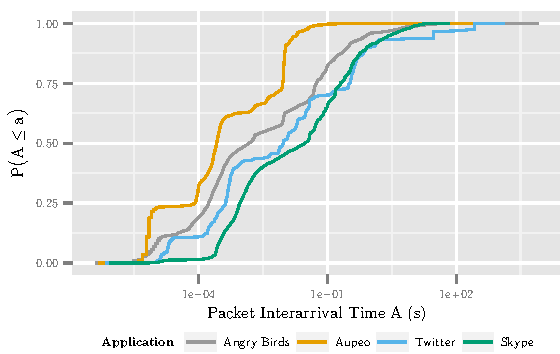
\includegraphics{network/network_traces/numerical_results/figures/interarrival_times}
\caption{CDF of interarrival times for considered applications}\label{fig:network:network_traces:numerical_results:traffic:interarrival_times}
\end{figure}

\begin{table}
  \centering
  \caption{Mean and standard deviation of interarrival time and bandwidth for considered applications}
  \label{tab:network:network_traces:numerical_results:traffic_statistics}
  \begin{tabular}{lcccc}
  	\toprule
    Application&\multicolumn{2}{c}{Interarrival time (\si{\second})}&\multicolumn{2}{c}{Bandwidth (\si{\kilo\bit\per\second})}\\
    \cmidrule(lr){2-3}\cmidrule(lr){4-5}
    &Mean&Standard deviation&Mean&Standard deviation\\
    \midrule
    Angry Birds&0.66 &15.90 & 4.42 & 4.50\\
    Aupeo&0.06 & 3.06& 129.76 & 482.63\\
    Twitter& 8.91&44.09 & 0.27 & 0.04\\
    Skype& 0.55 &1.95 & 1.30 & 1.84\\
    \bottomrule
  \end{tabular}
\end{table}

\paragraph*{Angry Birds}
We see that there are no distinct peaks in interarrival time, which would indicate a periodic behaviour.
Furthermore, we see that \SI{5}{\percent} of all interarrival times are greater than \SI{1}{\second}.
As we consider only \gls{TDCH} values above \SI{1}{\second}, those are candidates for triggering state transitions.
The mean interarrival time is \SI{0.66}{\second}, with a relatively high standard deviation of \SI{15.90}{\second}.
This is caused by the low interarrival times in one advertisement request at the beginning of each new level and the relatively large interarrival times between two advertisements.
Mean bandwidth is relatively low with \SI{4.42}{\kilo\bit\per\second} and a high standard deviation of \SI{4.5}{\kilo\bit\per\second}.
These differences can be explained by considering the behaviour of the application.
During long phases of use no traffic is sent, and after a level is restarted, a new advertisement has to be obtained, causing the transmission of data.
Note that no level data is downloaded during gameplay at all, as the complete game is downloaded during the installation process.

\paragraph*{Aupeo}
We see that the application generates packets with relatively small interarrival times with a small mean interarrival time of \SI{0.06}{\second}.
The high standard deviation of \SI{3.06}{\second} is caused by the wait between two tracks.
Furthermore, we see a high mean bandwidth of \SI{129.76}{\kilo\bit\per\second}, and a standard deviation of \SI{482.63}{\kilo\bit\per\second}.
This is caused by the difference in traffic activity between times when tracks are either downloaded or not.

\paragraph*{Twitter}
We see that \SI{90}{\percent} of all transmissions occur with an interarrival time of less than \SI{1}{\second}.
Also, we can observe a high mean interarrival time of \SI{8.91}{\second} and a high standard deviation of \SI{44.49}{\second}.
Additionally, the mean bandwidth is low with only \SI{0.27}{\kilo\bit\per\second} and a low standard deviation of \SI{0.04}{\kilo\bit\per\second} due to the fact that Twitter text messages are only \(140\) characters in length and thus only a low volume of traffic needs to be transmitted.

\paragraph*{Skype}
Similar to the Twitter application, we see that \SI{90}{\%} of all packets occur with an interarrival time of less than \SI{1}{\second}.
However, in contrast to Twitter, we see a low mean interarrival time of \SI{0.55}{\second} with a standard deviation of \SI{1.95}{\second}.
Further, we observe a relatively low mean bandwidth of \SI{1.30}{\kilo\bit\per\second} and a standard deviation of \SI{1.8}{\kilo\bit\per\second}.

\begin{figure}
\centering
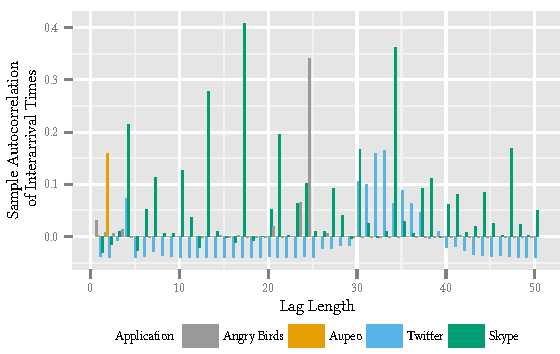
\includegraphics{network/network_traces/numerical_results/figures/autocorrelation}
\caption{Autocorrelation of interarrival times for considered applications}\label{fig:network:network_traces:numerical_results:traffic:autocorrelation}
\end{figure}

To further study the traffic patterns of the applications, we study the autocorrelation of the packet interarrival time with regard to the lag length in \reffig{fig:network:network_traces:numerical_results:traffic:autocorrelation}.
We note that all studied applications present completely different autocorrelations for the interarrival times.
This is one of the reasons that the applications under consideration will display different signalling behaviour in the next section.

\subsubsection*{Influence of Application Characteristics on Optimisation with Network Timers}\label{sec:network:network_traces:numerical_results:application_influence}
This section studies the impact of traffic generated by applications on both the network and the
\gls{QoE} of the user.
We consider two metrics.
First, we consider the frequency of signalling messages induced at network components such as an \gls{RNC}.
In light of network outages caused by so called signalling storms, a large number of signalling messages leading to overload at network equipment, it is in the interest of a network operator to reduce the number of signalling messages arriving at the \gls{RNC}.
One possible way to reduce the signalling frequency \gls{SF} is to modify network timer values, i.e., \gls{TDCH} and \gls{TFACH}.

As discussed in \refsec{sec:network:background:energy_consumption_qoe}, the \gls{QoE} a user perceives while using his device is influenced by the battery life of the \gls{UE}.
Thus, the second metric considered is the device’s power drain which is influenced by the used network model and associated timer settings.
As described in \refsec{sec:network:network_traces:calculating_metrics}, based on a measurement trace for an application we use \refalg{alg:network:network_traces:performance_evaluation:inferring_network_state:inference_algorithm} to infer the state transitions occurring during the use of the application.
Then, we calculate the relative time spent in each state and use \reftab{tab:network:network_traces:calculating_metrics:power_consumption} to compute the mean power
drain of the radio interface during the measurement.
We study both metrics, first on its own and then aggregated for both network models introduced in \refsec{sec:network:background:umts_rrc}.

In this section we first consider the Three State Model, which describes the default behaviour in \gls{3G} networks. 
Then, we describe the influence of the Two State Model which models a network behaviour similar to that if proprietary fast dormancy algorithms are used.
These algorithms have been identified as one of the causes of a signalling storm~\cite{NSN2011}.
Finally, we summarize the results and discuss the possible ramifications of using network timer values to reduce the signalling frequency.

\paragraph*{Three State Model: Signalling Frequency vs. Power Consumption}\label{sec:network:network_traces:numerical_results:three_states}
First, we investigate the signalling frequency generated by the studied applications for the three state network model. 
\reffig{fig:network:network_traces:numerical_results:three_states:three_states:signalling} shows the signalling frequency \gls{SF} with regard to the \gls{TDCH} timer.
\begin{figure}
	\centering
	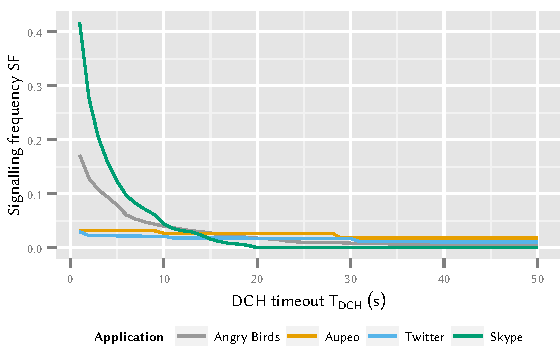
\includegraphics{network/network_traces/numerical_results/figures/3_state_tdch_vs_frequency}
	\caption{Signalling Frequency \gls{SF} for varying \gls{TDCH} timers for the Three State Model}\label{fig:network:network_traces:numerical_results:three_states:three_states:signalling}
\end{figure}
For all studies of the Three State Model, the \gls{TFACH} timeout is set to \(\gls{TFACH} = 2\cdot  \gls{TDCH}\), a realistic value as shown in \cite{Qian2011}.
We see that for \gls{TDCH} timers shorter than \SI{6}{\second} the Skype application in \gls{RRC_idle} mode generates the highest signalling frequency.
The Angry Birds application generates the second highest frequency of signalling messages, followed by the Aupeo application.
The Twitter application generates the smallest signalling frequency.
If the \gls{TDCH} value is longer than \SI{15}{\second}, this order changes.
However, in general the signalling frequency for higher \gls{TDCH} timeouts is lower than for shorter \gls{TDCH} timeouts.
Now, the Aupeo application has the highest signalling frequency, followed by the Twitter application.
The signalling frequency for the Angry Birds application takes the third place.
The application which generated the highest signalling frequency generates the lowest frequency for higher timeout values.
This behaviour can be explained by the fact that the Skype application sends keep-alive messages with an interval of less than \SI{20}{\second}.
If the timer is greater than the interval time of the keep-alive messages, the \gls{UE} stays always connected and thus generates almost no signalling.

These results show that the traffic patterns of the application have a large influence on the generated signalling frequency.
Signalling is generated for every pause in sending or receiving larger than the configured timeouts.
If such pauses occur frequently, this increases the signalling frequency as shown on the examples of Skype and Angry Birds.
Applications with more time between the sending or receiving of data cause less signalling, as shown by Aupeo and Twitter.
Furthermore, we can observe that the signalling frequency can be reduced by increasing the \gls{TDCH} timeout, with the minimum being reached as \gls{TDCH} approaches infinity.
From a signalling frequency perspective, a value of \SI{20}{\second} would probably be sufficient, however if other metrics such as radio resource consumption are considered \SI{10}{\second} would be acceptable for a network operator.

Based on this finding, we see that increasing the \gls{TDCH} timer decreases the signalling frequency \gls{SF} at the \gls{RNC}.
However, the actual signalling frequency depends on the application running at the \gls{UE}.
From a network operator's point of view, the Three State Model should always be preferred to the Two State Model because it generates less signalling messages per second, thus decreasing the load at the \gls{RNC}.
This view does however not consider the additional radio resources which are kept in use for a longer time if larger \gls{TDCH} values are used.
Additionally, it should be noted that the choice of the network model is sometimes outside of the domain of the network operator.
Proprietary Fast Dormancy algorithms, as the considered Two State Model, are enabled on the \gls{UE} by the user.

\begin{figure}
	\centering
	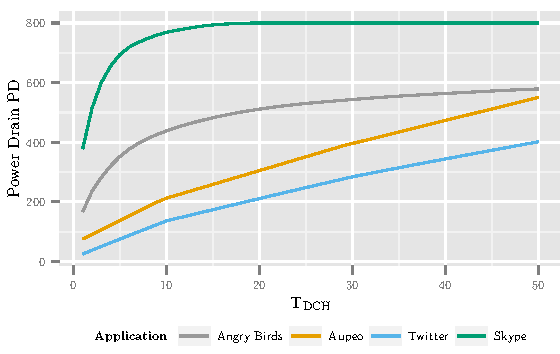
\includegraphics{network/network_traces/numerical_results/figures/3_state_tdch_vs_power_drain}
	\caption{Power Drain \gls{PD} for varying \gls{TDCH} timers for the Three State Model}\label{fig:network:network_traces:numerical_results:three_states:power_drain}
\end{figure}
In \reffig{fig:network:network_traces:numerical_results:three_states:power_drain} we consider the power drain if the network uses the Three State Model, i.e. if the Fast Dormancy mode of the \gls{UE} is disabled.
The figure shows the mean power drain \gls{PD} of the device with regard to the \gls{TDCH} timeout.
Possible values range between \SI{0}{\milli\watt} if the \gls{UE} was in \gls{RRC_idle} state during the whole measurement and \SI{800}{\milli\watt} if the \gls{UE} was in \gls{RRC_DCH} state during the complete measurement.
We see that the least power over all considered \gls{TDCH} values is consumed by the Twitter application.
The second least power drain is required by Aupeo, followed by Angry Birds.
Finally, the most power is consumed by Skype.
Here we see that the maximum value of \SI{800}{\milli\watt} is reached at a \gls{TDCH} timeout of \SI{20}{\second}.
This is because, due to the periodic traffic behaviour of Skype, the device is always in \gls{RRC_DCH} state.
Again, we see that the traffic characteristics of the applications impact the power drain.
Applications with more network activity are forced to stay in more power consuming states for a longer time.
We see that for very small network timers, the power drain is minimal.
However, as seen in the last section small timers increase the signalling frequency at the \gls{RNC}.
Again, a choice of \SI{10}{\second} for the \gls{TDCH} timer can be seen as a compromise between signalling frequency \gls{SF} and power drain \gls{PD}.

\begin{figure}
	\centering
	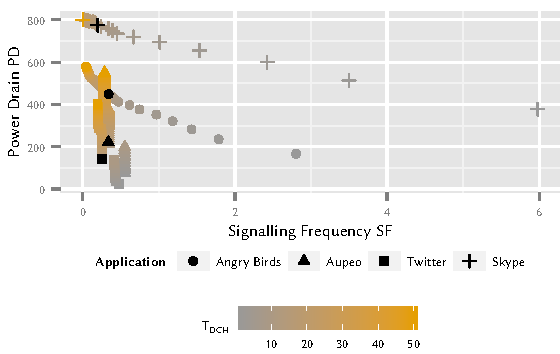
\includegraphics{network/network_traces/numerical_results/figures/3_state_signalling_vs_power_consumption}
	\caption{Influence of manipulating \gls{TDCH} timer on Signalling Frequency \gls{SF} and Power Drain \gls{PD} for the Three State Model. Filled marker highlights \(\gls{TDCH} = \SI{11}{\second}\)}\label{fig:network:network_traces:numerical_results:three_states:trade_off}
\end{figure}
Finally, we aggregate both metrics in in \reffig{fig:network:network_traces:numerical_results:three_states:trade_off}.
The X-axis of the figure gives the signalling frequency.
On the Y-axis we show the power drain \gls{PD}.
Different \gls{TDCH} values are shown by different colors as specified by the colorbar.
First, we consider Angry Birds.
We observe that as the signalling frequency approaches zero, the power drain rapidly increases, even if only small gains in signalling frequency reduction can be achieved.
The Aupeo application presents a completely different picture.
Here, we can see multiple almost horizontal lines of markers.
If \gls{TDCH} is chosen in this range, each increase of \gls{TDCH} brings a small decrease in signalling frequency \gls{SF} for a increase in power drain \gls{PD}.
However, some points of discontinuity exist.
If for example the \gls{RRC_DCH} timer is increased from \SI{10}{\second} to \SI{11}{\second}, a decrease in signalling frequency \gls{SF} of \SI{40}{\percent} can be achieved by only suffering from a small increase in power drain.
These points of discontinuity would present themself to be suitable targets of optimisation.
Next, we consider the Twitter application.
It displays a similar behaviour as the Aupeo application, with multiple points of discontinuity.
Note that Twitter exhibits a different point of discontinuity, and the \gls{TDCH} value of \SI{10}{\second}, which provided good results for Aupeo is not optimal for Twitter.
Finally, Skype again shows a completely different picture then all the other considered applications.
First, note that due to the large signalling frequency \gls{SF} of Skype for small values of \gls{TDCH}, \(\gls{TDCH} = \SI{1}{\second}\) is not displayed in the figure.
Furthermore, as the \gls{TDCH} timer increases above \SI{20}{\second} the signalling frequency \gls{SF} does not decrease any further, and the power drain \gls{PD} remains at the maximum value.
We observe that there is no common optimal value for all applications which would result in an acceptable tradeoff.


\paragraph*{Two State Model: Signalling Frequency vs. Power Drain}\label{sec:network:network_traces:numerical_results:two_states}
Now, we study the consequences of the application traffic in a network using the Two State Model.
The Two State Model occurs in reality if Fast Dormancy implementations are considered.
Here, the \gls{UE} disconnects from the network if for a certain time no traffic is sent or received in order to reduce power drain.
\begin{figure}
	\centering
	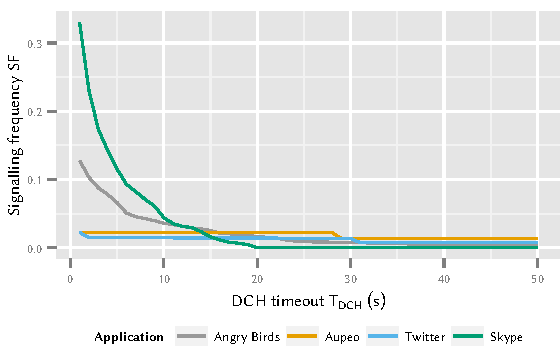
\includegraphics{network/network_traces/numerical_results/figures/2_state_tdch_vs_frequency}
	\caption{Signalling Frequency \gls{SF} for varying \gls{TDCH} timers for the Two State Model}\label{fig:network:network_traces:numerical_results:two_states:signalling}
\end{figure}
As for the Three State Model, \reffig{fig:network:network_traces:numerical_results:two_states:signalling} shows the signalling frequency \gls{SF} with regard to the setting of the \gls{TDCH} timer.
We see the same general behaviour as with the Three State Model, however the signalling frequency generated by each of the applications for the Two State Model are usually higher.
For example, even for relatively high \gls{TDCH} timeout values of \SI{10}{\second}, the Angry Birds application causes \SI{270}{\percent} of the signalling frequency \gls{SF} as in a network using the Three State Model.

\begin{figure}
	\centering
	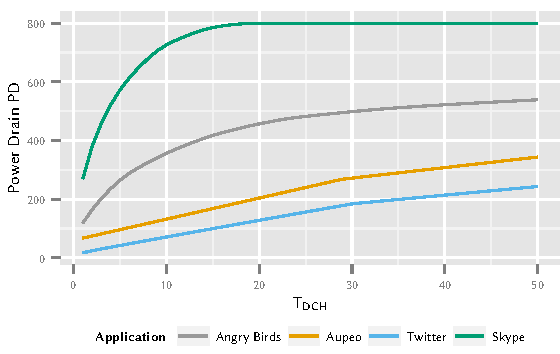
\includegraphics{network/network_traces/numerical_results/figures/2_state_tdch_vs_power_drain}
	\caption{Power Drain \gls{PD} for varying \gls{TDCH} timers for the Two State Model}\label{fig:network:network_traces:numerical_results:two_states:power_drain}
\end{figure}
Next, we consider the changes in the power drain of the \gls{UE} if the user decides to enable Fast Dormancy, i.e. switch to a Two State Model, in \reffig{fig:network:network_traces:numerical_results:two_states:power_drain}.
As with the signalling frequency, we only see a quantitative difference to the Three State Model.
Again, we compare the differences between Two State Model and Three State Model on the example of the Angry Birds application.
For the same considered \gls{TDCH} timeout of \SI{10}{\second}, we see a decrease of \SI{81}{\percent} in power drain \gls{PD} when compared with the Three State Model.

\begin{figure}
	\centering
	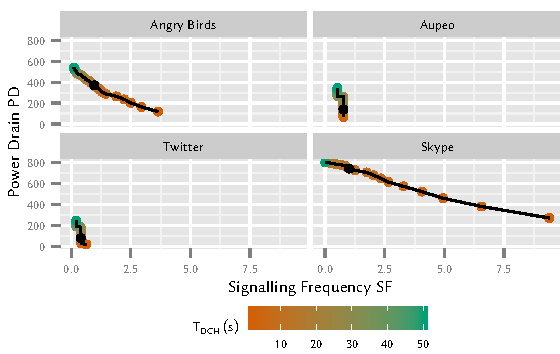
\includegraphics{network/network_traces/numerical_results/figures/2_state_signalling_vs_power_consumption}
	\caption{Influence of manipulating \gls{TDCH} timer on Signalling Frequency \gls{SF} and Power Drain \gls{PD} for the Two State Model. Filled marker highlights \(\gls{TDCH} = \SI{11}{\second}\)}\label{fig:network:network_traces:numerical_results:two_states:trade_off}
\end{figure}
Finally, we compare the influence of changes of thr \gls{TDCH} timeout on both signalling frequency \gls{SF} and power drain \gls{PD} for the Two State Model in \reffig{fig:network:network_traces:numerical_results:two_states:trade_off}.
As for the Three State Model, we see that there is no tradeoff between power drain and signalling frequency which would be acceptable for all application.
Even for single applications \gls{TDCH} values such as \SI{10}{\second} which was an acceptable tradeoff Angry Birds is no longer a good choice in the Two State Model.

\subsubsection*{Consequences of Trade-Off: Signalling Frequency vs. Power Consumption}\label{sec:network:network_traces:numerical_results:trade_off}

In order to illustrate the impact of the behaviour discussed in the previous section, we compare the influence of the \gls{TDCH} timer on an application with different traffic characteristics, for example the Aupeo application as shown in \reffig{fig:network:network_traces:numerical_results:consequences:aupeo}.
\begin{figure}
	\begin{subfigure}[b]{.5\textwidth}
	\centering
	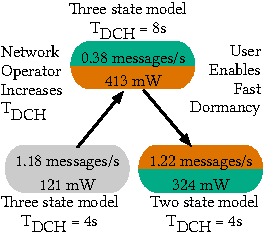
\includegraphics{network/network_traces/numerical_results/figures/consequences_angry_birds}
	\caption{Angry Birds}\label{fig:network:network_traces:numerical_results:consequences:angry_birds}
	\end{subfigure} 
	\begin{subfigure}[b]{.5\textwidth}
	\centering
	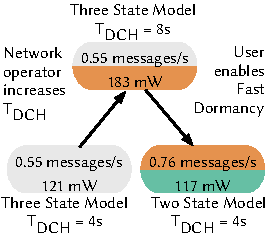
\includegraphics{network/network_traces/numerical_results/figures/consequences_aupeo}
	\caption{Aupeo}\label{fig:network:network_traces:numerical_results:consequences:aupeo}
	\end{subfigure}

	\caption{Influence of manipulating \gls{TDCH} timer on different applications}\label{fig:network:network_traces:numerical_results:consequences}
\end{figure}
The signalling frequency \gls{SF} before the increase of the \gls{TDCH} timer was \(0.55\) messages per second, after the change to \(\gls{TDCH} = \SI{8}{\second}\) the signalling frequency remains unchanged.
Thus, the policy change based on one application brings no significant gain to other applications.
However, from a user's point of view, the power drain \gls{PD} increased from \SI{121}{\milli\watt} to \SI{183}{\milli\watt}.
Again, we assume the user activates fast dormancy to deal with the increase in power drain of more than $50\%$.
This results in a decrease of power drain \gls{PD} to \SI{117}{\milli\watt}, and an increase of overall signalling frequency \gls{SF} to \(0.76\) messages per second.
By changing the value without considering all applications, the network operator has decreased the \gls{QoE} for other users, and worsened his overall situation.
Thus, due to the large number of applications it seems impossible to optimise the \gls{TDCH} timeout to reduce the signalling frequency without negatively impacting the users \gls{QoE} in unexpected ways.

There exist applications, like Twitter and Aupeo, where optimisation by modifying the \gls{TDCH} values can provide acceptable results.
However, these optimisations are only successful if a single application or network model is considered.
For other applications, like Angry Birds or Skype, this optimisation approach does not seem to be successful.
A reduction of signalling frequency and power drain is possible, if the application developers are incentivised to optimise their applications in these regards.
In \cite{Qian2011} the authors suggest methods to achieve this optimisation, for example batch transfer of advertisements for applications like Angry Birds or decreasing the refresh rate in applications like Skype.
However, at the moment application developers are neither receiving incentives to optimise applications in this way, nor do hardware vendors provide interfaces to facilitate such optimisation.
Such interfaces would allow application developers to schedule their data transmissions in such a way that both signalling and battery drain would be reduced.
Additionally, these interfaces would need to allow the application developer to specify whether sending the transmission is urgent.
One example of such urgency would be if the application is being actively used by the user and requires the feedback of the transmission.
If the data is being sent as a regular update while the application is running in the background it could be scheduled for later transmission as suggested by \cite{calder2010, vergara2012}.

\subsection{Influence of Network Configuration and Background Traffic on Web QoE}\label{sec:network:network_traces:numerical_results:web_qoe}
So far we have discussed only power drain as a \gls{QoE} influence factor.
For applications like web browsing, one relevant QoE influence factor are page load times.
Therefore, we consider a web QoE model which quantifies the impact of page load times on mean opinion scores \cite{egger2012a}.
We distinguish here between \emph{web \gls{QoE}} and \emph{\gls{QoE}}, as no \gls{QoE} models are currently existing which consider page load times as well as power drain.
In this section, we study the impact of background traffic as well as network timer settings on the page load time of an image and the resulting \gls{MOS}.
For this study, we only consider the three state network model, but the results can be applied to the 2-state model as well.

We assume a scenario, where a user is running a background application like Twitter or Skype.
Then, while the application is in the background, the user begins to download an image from a website.
Due to the background traffic, and depending on the network model and associated timer values, the \gls{UE} may be currently either in \gls{RRC_idle}, \gls{RRC_FACH} or \gls{RRC_DCH} state.
We give the probability of a random observer encountering the system in \gls{RRC_FACH} state by \(p_{\gls{RRC_FACH}}\) and the probability of a random observer encountering in \gls{RRC_idle} state by $p_{\gls{RRC_idle}}$.
If the device is currently not in \gls{RRC_DCH} state, it takes some time to connect.
This promotion time depends on the current state and is according to \cite{Qian2010b} \SI{2}{\second} if the \gls{UE} is in \gls{RRC_idle} state and \SI{1.5}{\second} if the device is in \gls{RRC_FACH} state.
For this study, we assume that the user randomly chooses a time to begin downloading an image.
The time until the image is displayed consists of the time to load the page \(t_p\), as well as the time to go online \(t_o\), where \(t_o\) is the mean time to go online, given as 
\[t_o = p_{\gls{RRC_idle}} \cdot \SI{2.5}{\second} + p_{\gls{RRC_FACH}} \cdot \SI{1.5}{\second}.\]
In reality, an additional delay is added due to the latency of the physical display, however as this happens in a smaller timescale we neglect it in this model.
Thus, the total time \(t\) that is required to download the image is given by \(t = t_o + t_p\).

The authors of \cite{egger2012a} give a function to calculate the \gls{MOS} based on the required page load time as \(QoE(t) = a\cdot \ln t + b\), were \(a\) and \(b\) depend on the type of content being downloaded.
For our scenario, picture download, values of \(a = -0.8\) and \(b = 3.77\) are suggested.
It has to be noted that for different web sites, the logarithmic function was still observed, but different values for \(a\) and \(b\) were obtained as given in \cite{egger2012a}.
These values depend for example on the type of web page as well as the size of the content.
Nevertheless, the results presented in this section are therefore generalizable for web browsing to various pages.
This allows us to give an expected \gls{MOS} for downloading pictures while a background application is influencing the probability of a device already being in \gls{RRC_DCH} state or still having to be promoted to \gls{RRC_DCH} state.

\begin{figure}
	\begin{subfigure}[b]{\textwidth}
	\centering
	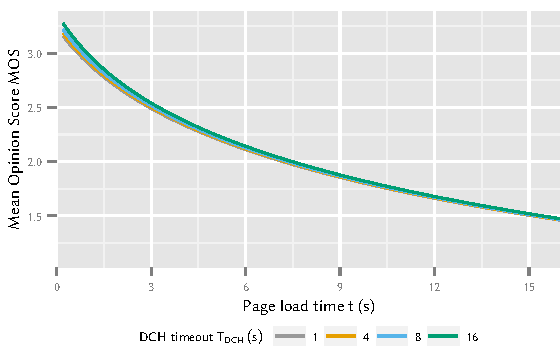
\includegraphics{network/network_traces/numerical_results/figures/qoe_with_backgroundapp_twitter}
	\caption{Background traffic generated by Twitter}\label{fig:network:network_traces:numerical_results:web_qoe:twitter}
	\end{subfigure} 

	\begin{subfigure}[b]{\textwidth}
	\centering
	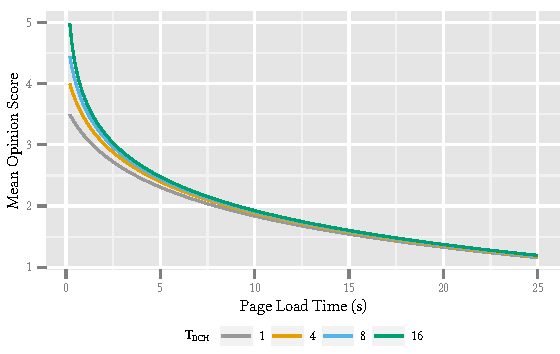
\includegraphics{network/network_traces/numerical_results/figures/qoe_with_backgroundapp_skype}
	\caption{Background traffic generated by Skype}\label{fig:network:network_traces:numerical_results:web_qoe:skype}
	\end{subfigure}

	\caption{Perceived Web-\gls{QoE} for loading a page with existing background traffic}\label{fig:network:network_traces:numerical_results:web_qoe}
\end{figure}

Using this methodology, we study the influence of background traffic on the \gls{QoE} for two background applications with different traffic characteristics.
In \reffig{fig:network:network_traces:numerical_results:web_qoe:twitter} we assume that the user is running the Twitter application as a background process.
The application is set to update the users status feed every \SI{300}{\second}.
In \reffig{fig:network:network_traces:numerical_results:web_qoe:skype} the user is running the Skype application as a background application.
This application sends keep alive messages every \SI{20}{\second}.
For each application, we assume the three state network model with \gls{TDCH} settings of \SIlist{1;4;8;16}{\second}.
We always set \(\gls{TFACH} = 2\cdot \gls{TDCH}\).
In both figures we show the assumed page load time, as provided by the network, on the X-axis for values from \SIrange{0.2}{25}{\second}.
We assume \SI{0.1}{\second} as a lower bound because page load times lower than \SI{0.1}{\second} seconds are not distinguishable \cite{egger2012b} by humans.
The calculated \gls{MOS} values are given on the Y-Axis.

The picture downloads with the background traffic generated by the Twitter application result in \gls{MOS} values beginning at \(3.15\) for \(\gls{TDCH} = \SI{1}{\second}\), \(3.18\) for \(\gls{TDCH} = \SI{4}{\second}\), \(3.21\) for \(\gls{TDCH} = \SI{8}{\second}\), and \(3.27\) for \(\gls{TDCH} = \SI{16}{\second}\) respectively.
With increasing page load time, the \gls{MOS} again decreases.
This behaviour is due to the fact that the Twitter application periodically sends traffic every \SI{300}{\second}.
Then, no further activity occurs until the next refresh occurs.
In this time, the \gls{UE} transitions to \gls{RRC_idle} state.
This traffic characteristic causes a high probability of a user encountering the device in a \gls{RRC_idle} state.
Additionally, the traffic characteristics of the background application show that different \gls{TDCH} settings impact the web \gls{QoE} only marginally, resulting in the lines in the graph being grouped close together.

In contrast, downloading pictures with the Skype application generating background traffic, causes different \gls{MOS} values.
For a page load time of \SI{0.2}{\second} the \gls{MOS} value with \(\gls{TDCH} = \SI{1}{\second}\) is \(3.49\) with \(\gls{TDCH} = \SI{4}{\second}\) we get \(3.99\) for \(\gls{TDCH} = \SI{8}{\second}\) we get a \gls{MOS} value of \(4.44\) and finally for \(\gls{TDCH} = \SI{16}{\second}\) we get \(4.99\) respectively.
For increasing page load times, the \gls{MOS} decreases.
This increased \gls{MOS} values occur because of the high frequency of traffic sent by the Skype application.
Here, every \SI{20}{\second} traffic is sent.
This means that even for relatively low values of \(\gls{TDCH}\) the user has a high probability of encountering a state where no promotion delay is required before the actual page load time can begin.

From these studies we can conclude that, when considering \gls{QoE} on mobile devices, not only the page load time caused by the network but also additional delays caused by the state of the device should be considered.
As shown on two examples, this state can be affected by other applications which are running in the background and generate traffic.


